\section{Konzeption des neuen Krabbelroboters}
\label{sec:konzeption}

Im folgenden Abschnitt wird der Zustand des Projekts bei der Übernahme beschrieben, sowie die Zielsetzungen, die sich daraus ergeben. Außerdem werden die Vorgehensweisen dargelegt, die für die Umsetzung jener Ziele geplant sind.

\subsection{Mechanischer Aufbau und Konstruktionsprinzipien}

\subsubsection{Analyse des Ausgangsmodells}

Zu Beginn des Projekts wird der einarmige Krabbelroboter des Vorgängerprojekts in Bezug auf Software, Hardware und Funktionsumfang analysiert. Dazu wird besonders die Dokumentation des Vorgängerprojekts angesehen \cite{vorgängerprojekt}.

\textbf{Mechanische Analyse}

Der Roboter wurde dabei einer mechanischen Strukturanalyse unterzogen. Er bestand zum Zeitpunkt der Übernahme aus einer Basis (Chassis) mit einem Arm (Motor 1) und einer Hand bzw. Greifer (Motor 2). Die drei Bauteile sind mit je einem Rotationsgelenk, also insgesamt zwei Gelenken, miteinander verbunden. Die Gelenke wurden durch Dynamixel-Servos dargestellt. Der Aufbau lässt sich also als Kinematische Kette darstellen.

% Daher konnte die Anzahl $n$ an Freiheitsgraden (DoF) des Roboters mit der Formel von Grübler berechnet werden. Ein Freiheitsgrad ist dabei \glqq jede verbleibende unabhängige Bewegungsfreiheit eines Systems\grqq \ \cite{robotik_scriptum}.
% \begin{align}
%   n = m \cdot (N - 1 - J) + \sum_{i=1}^{J}f_i \noindent \\
%   n = 6 \cdot (3 - 1 - 2) + \sum_{i=1}^{2}1 = 6 \cdot 0 + 2 = 2
% \end{align}
% Dabei ist \glqq $m$ die Anzahl der Freiheitsgrade jedes Starrkörpers ($m = 6$ im dreidimensionalen Raum)\grqq \ \cite{robotik_scriptum}, $N$ die Anzahl der Starrkörper (hier 3: Chassis, Arm, Hand), $J$ die Anzahl der Gelenke (hier 2) und $f_i$ die Anzahl an Freiheitsgraden des Gelenks $i$. 

% Des Weiteren wurde die Form des Konfigurationsraum des Roboters untersucht. Der Konfigurationsraum beschreibt alle möglichen Positionen und Orientierungen des Roboters im Raum. Mit der Form ist seine topologische Struktur gemeint, sprich wie die möglichen Konfigurationen (alle Konfigurationen zusammen ergeben den Konfigurationsraum) zusammenhängen. Da der Krabbel-Roboter zwei zyklische Rotationsgelenke hat, ergibt sich die Form eines zweidimensionalen Torus $(T^2 = S^1 \times S^1)$, wobei $S^1$ die Menge aller Punkte auf einem Kreis darstellt \cite{robotik_scriptum}. Abbildung \ref{fig:torus} zeigt dies visuell.
% \begin{figure}[h]
%   \centering
%   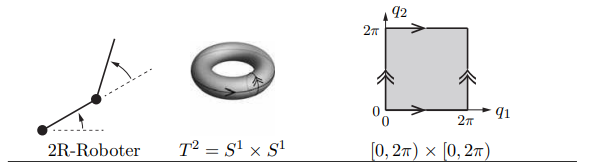
\includegraphics[width=0.7\textwidth]{torus.png}
%   \caption{Der Konfigurationsraum des Krabbelroboters als Torus, aus \glqq Grundlagen der Robotik\grqq \ \cite{robotik_scriptum}.}
%   \label{fig:torus}
% \end{figure}

% Das Robotersystem entspricht also einem (autonomen) mobilen Roboter mit 2 DoF und einem planaren 2R-Roboterarm. Daraus ließe sich eine Kinematische Modellierung bzw. Simulation erstellen, die allerdings nicht im Rahmen dieser Abschlussarbeit angefertigt wurde. 

\textbf{Funktionsumfang}

Der Funktionsumfang des Roboters beschränkte sich auf die Steuerung der Motoren, um den Arm bzw. die Hand über eine graphische Benutzeroberfläche (GUI) zu bewegen.

\subsubsection{CAD-gestütztes Design und 3D-Druck}

Die Bauteile und das Gehäuse des Roboters wurden mithilfe eines CAD-gestützten Entwicklungsprozesses mit \emph{Autodesk Fusion 360} \cite{fusion360} erstellt. Die digitale Modellierung ermöglichte eine präzise Gestaltung der Bauteile, die direkt überprüft werden konnten. Für den Austausch und die Weiterverarbeitung (insbesondere mit Herrn Prof. Dr. Ihme) wurden die Modelle als standardisierte STEP-Dateien exportiert.

Der anschließende 3D-Druck der Komponenten erlaubte eine einfache, schnelle und kostengünstige Fertigung. Durch das additive Herstellungsverfahren wurde nur das tatsächlich benötigte Material eingesetzt, was sowohl Gewicht als auch Ressourcen sparte. Besonders vorteilhaft am Prozess ist zudem, dass keine komplexen Werkzeuge oder Maschinen notwendig sind. Für die Entwicklung wird lediglich ein Computer benötigt, wodurch es wesentlich unkomplizierter ist, Änderungen umzusetzen.

Der kombinierte CAD- und 3D-Druckprozess unterstützt somit eine iterative und flexible Entwicklung, wie sie im Prototypenbau von mobilen Robotern besonders hilfreich ist.

\subsubsection{Gestaltungsschwerpunkte}

Ziel der Weiterentwicklung des übernommenen einarmigen Krabbelroboters war es, ein modular aufgebautes, leichtes und anschaulich gestaltetes System zu schaffen, das sowohl für Demonstrations- als auch Auswertungszwecke geeignet ist. Dabei wurden folgende Anforderungen von uns anfangs festgelegt:

\textbf{Must-Have}
\begin{itemize}
  \item \textbf{Modularität (Basic):} Das Austauschen oder Erweitern zentraler Komponenten (insbesondere des Akkus) sollte erleichtert werden, etwa durch Steck- oder Schraubverbindungen.
  \item \textbf{Offenes Design:} Für Demonstrationszwecke müssen alle Komponenten sichtbar und gut zugänglich montiert sein, um einen schnellen Überblick über das System zu ermöglichen.
  \item \textbf{Verbesserter Schwerpunkt:} Damit das Bein möglichst wenig Last stemmen muss, sollte ein Schwerpunkt nah an der Radachse angestrebt werden.
  \item \textbf{Leichtbauweise:} Ein geringes Gewicht unterstützt die Energieeffizienz und erleichtert die Steuerung durch kleinere Antriebsmotoren.
  \item \textbf{Mechanische Kompatibilität:} Es muss auf die Verwendung standardisierter Bauteile (z.\.B. M3/M4-Schrauben) geachtet werden, um einfache (De-)Montage und Erweiterbarkeit sicherzustellen.
\end{itemize}

\textbf{Nice-to-Have}
\begin{itemize}
  \item \textbf{Kabelmanagement:} Ordnung und Übersicht im Innenraum durch Führungen oder Halteclips.
  \item \textbf{Klicksysteme:} Gehäuseteile, die ohne Werkzeug geöffnet oder getauscht werden können.
  \item \textbf{Kühlung und Luftzirkulation:} Ein passives oder aktives Kühlsystem angestrebt (Besonders für den Raspberry Pi).
\end{itemize}

\textbf{Optional}
\begin{itemize}
  \item \textbf{Autonomiefunktionen:} z.\.B. selbstständige Navigation zur Erweiterung des Funktionsumfangs.
  \item \textbf{Erweiterte Sensorik:} Zusätzliche Sensoren wie LiDAR als langfristige Option.
  \item \textbf{Symmetrisches Design:} Eine symmetrische Gestaltung kann die Bewegungsvorhersagbarkeit erhöhen und die Konstruktion vereinfachen.
  \item \textbf{Diagnoseelemente:} LEDs oder Displays zur Anzeige von Systemzuständen (wie etwa Spannung, Kommunikation, Fehlermeldungen) zur Ergänzung der bestehenden, digitalen Lösungen.
\end{itemize}

Diese Zielkriterien bildeten die Grundlage für die Auswahl der Bauteile einschließlich Akku und das mechanische Design des weiterentwickelten Roboters.

\subsection{Software}

Die Architektur der Crawler-Software, also die Strukturierung des Codes, war einer der wichtigsten Verbesserungspunkte im Vergleich zum Vorgängerprojekt (im Folgenden mit "Legacy-" bezeichnet). 

\subsubsection{Upgrade von ROS 1 zu ROS 2}

Im Vergleich zur Legacy-Codebase portierten wir das Projekt von ROS 1 zu ROS 2. ROS 2 ist zum Zeitpunkt der Arbeit die neueste Major-Version von ROS und unterstützt modernere Versionen des Ubuntu-Betriebssystems. Dadurch konnten wir das Betriebssystem auf dem Raspberry Pi von Ubuntu 18.04 auf Ubuntu 24.04 upgraden. Support für ROS 1 endete außerdem im Mai 2025, während der Laufzeit des Projekts, und die Legacy-installation hätte keine Updates mehr erhalten. Das Upgrade von ROS 1 auf ROS 2 erfordert einige grundlegendere Veränderungen an einem ROS-Projekt, da wir aber ohnehin eine vollständige Überarbeitung der Codebase anstrebten, bedeutete dies praktischerweise keinen zusätzlichen Aufwand. 

\subsubsection{Developer Experience}

An vorderer Stelle, sowohl in unserer Priorisierung als auch chronologisch im Projektverlauf, stand auch die Verbesserung der Developer Experience (DX), also eine bewusste Investition in einen reibungslosen Entwicklungsprozess, die mit einer geringeren Fehleranfälligkeit, erhöhtem Komfort und einer gesteigerten Entwicklungsgeschwindigkeit für uns und mögliche nachfolgende Teams einhergeht. 

Das Legacy-Projekt verfolgte dies bereits mit einem teilweisen Umstieg von Versionskennzeichnungen im Dateinamen zu einer üblichen Versionskontrolle mit Git. Das führten wir weiter und nutzten GitHub zur einfachen Kollaboration. 

\textbf{Synchronisierung des Quellcodes}

Im Legacy-Projekt wurde der Programmcode direkt auf dem Raspberry Pi entwickelt, der den Roboter steuert. Wir wollten es ermöglichen, den Code lokal etwa auf dem eigenen Laptop zu editieren, um dabei eine vollwertige Entwicklungsumgebung und andere Tools verwenden zu können, für die die Leistung des Raspberry Pi nicht ausreicht. Außerdem ist dies eine logistische Erleichterung, indem der Pi nun während der Entwicklung und des Betriebs nie zwingend an einen Bildschirm angeschlossen werden muss, und mehrere Personen gleichzeitig daran arbeiten können. 

Die Synchronisierung des Codes vom Endgerät auf den Pi erfolgt via SSH oder FTP, wobei \texttt{rsync} für eine beschleunigte Synchronisierung durch das Überspringen unveränderter Dateien genutzt wird. Es muss also eine TCP-Verbindung zum Raspberry Pi bestehen, die etwa durch ein lokales Netzwerk, unterwegs durch einen mobilen Hotspot oder auch remote durch eine Portfreigabe hergestellt werden. Eine weitere Option ist die Nutzung eines SSH Reverse Tunnels über einen öffentlichen Anbieter, wodurch lediglich der Internetzugriff durch den Pi und nicht der direkte externe Zugriff auf den SSH-Port des Pi nötig ist, was ggf. unmöglich ist. 

Die Notwendigkeit einer Internetverbindung ist eine zusätzliche Unannehmlichkeit, die sich jedoch auszahlen dürfte, da der Pi so nicht über einen Bildschirm verfügen muss, indem das Ausführen der ROS-Startbefehle via SSH und der Zugriff auf das Webinterface via HTTP von einem externen Gerät aus geschieht; jederzeit kann stattdessen auch ein Bildschirm und eine Tastatur angeschlossen werden, um Entwicklung und Betrieb wie gewohnt offline zu ermöglichen. 

\textbf{Vereinfachter Entwicklungszyklus mit Pixi}

Pixi ist ein Tool zur Softwareentwicklung, das die Verwaltung von Software-Bibliotheken vereinfacht und gleichzeitig als Build-System dient. Bibliotheken und Build-Befehle werden von Pixi in einer Textdatei im Projektverzeichnis gespeichert, sodass die gesamte Entwicklungsumgebung unabhängig vom Hostsystem reproduzierbar ist.

Der Entwicklungszyklus besteht aus mehreren Schritten, die notwendig sind, um das Programm auf dem Roboter auszuführen:
\begin{itemize}
	\item Der gesamte Quellcode muss auf den Raspberry Pi synchronisiert werden.
	\item Die Web-Komponente wird mithilfe von npm, einem Build-Tool für JavaScript, zu einer statischen HTML-Datei gebaut. Da dies auf dem Pi ziemlich lange dauert, kann die Web-Komponente auch zuerst lokal auf dem eigenen Rechner gebaut werden, damit die resultierende HTML-Datei direkt auf den Pi synchronisiert werden kann.
	\item Diese HTML-Datei und der Rest des Programms werden mithilfe von ROS zu einem ausführbaren Programm gebündelt.
	\item Dieses Programm wird mit einem ROS-Befehl gestartet.
\end{itemize}

Mit Pixi konnten wir diesen mehrschrittigen Build-Prozess auf dem Roboter stark vereinfachen. Die einzelnen Schritte sind in Pixi-Befehlen wie \texttt{pixi run upload} oder \texttt{pixi run build-web} definiert, was die Arbeit mit der Codebase wesentlich erleichtert. Im Vergleich zum Vorgängerprojekt ist es außerdem nun leichter, den Build-Prozess zu dokumentieren und zu überliefern. Die Befehle zum Starten des Legacy-Programms mussten uns bei der Projektübergabe noch mündlich mitgeteilt werden, da sie in der Legacy-Codebase nicht festgehalten waren. 

\textbf{Python Type Hints}

Ein weiterer Schritt in der Verbesserung der Developer Experience war das Hinzufügen sogenannter Type Hints in der Python-Codebase. Als Programmiersprache mit dynamischen Typen passieren in Python schnell Fehler, wenn Variablen bezüglich ihres Typs falsch verwendet werden.

Der folgende Python-Code produziert bei seiner Ausführung eine Fehlermeldung wegen falsch verwendeter Typen:

\begin{minted}{python}
def greet(s):
	# An dieser Stelle entsteht ein "TypeError".
	return "Hello " + s

greet(1)
\end{minted}

Diese Fehlermeldung kann wegen der dynamischen Funktionsweise von Python jedoch erst während der Ausführung des Programms entdeckt werden. Type Hints können in einer Codebase hinzugefügt werden, um diese Art der Fehler automatisch zu finden und zu korrigieren, ohne dass eine Ausführung des Programms notwendig ist. Durch entsprechendes Tooling in der Arbeitsumgebung kann dieser Prozess nahtlos in den Entwicklungsprozess integriert werden.

Im gezeigten Python-Code sähen Type Hints folgendermaßen aus:

\begin{minted}{python}
def greet(s: str) -> str:
	return "Hello " + s

greet(1)
\end{minted}

Die hinzugefügten Type Hints geben an, dass die Variable \texttt{s} vom Typ String sein muss, sowie, dass die \texttt{greet}-Funktion einen String als Output produziert.

Wir nutzten mypy \cite{mypy}, um die Nutzung von Type Hints strikt durchzusetzen und von ihnen im Entwicklungsprozess Gebrauch zu machen.

\subsubsection{Architektur der ROS-Nodes}

%- Architektur als Hauptverbesserungspunkt
%- wie es davor war:
%  - fehlende Sortierung zwischen Scripts, Backend-Code, Frontend-Code
%  - zwar verschiedene Nodes, aber trotzdem z.B. Hardware-Steuerung Teil der q_learning-Node etc.
%- wieso die Nodes aufgeteilt sind (anders als zuvor)
%- welche Nodes und Topics existieren, in welchem Verhältnis sie zueinander stehen:
%  - Hardware-Nodes, Web API; crawler_rl_environment, crawler_q_learning; crawler_rl_environment als Interface zwischen RL-Welt und Hardware-Welt
%  -> Diagramm

Die Verbesserung der Codebase zeigt sich vor allem in der Architektur der ROS-Nodes. In der Legacy-Codebase fanden wir initial eine Datei- und Codestruktur vor, die unseren persönlichen stilistischen Präferenzen nicht vollständig entsprach. Insbesondere in der Umsetzung einer für ROS-Applikationen idiomatischen Aufteilung in mehrere Nodes sahen wir Verbesserungspotenzial, da bspw. Code zur konkreten Hardwaresteuerung nicht von der Implementation des Q-Learning-Algorithmus abgegrenzt und teilweise mehrfach dupliziert war. Neben dem zusätzlichen Aufwand, der mit dem Weiterentwickeln einer unbekannten Codebase immer verbunden ist, waren diese stilistischen und architektonischen Differenzen mit der Legacy-Codebase, die nicht schwerwiegend oder unlösbar, aber weitreichendend waren, der Grund für unsere Entscheidung, die Crawler-Software unter Zuhilfenahme des existierenden Codes von Grund auf neu zu schreiben. 

Der neuen Architektur liegt, insbesondere im Vergleich zum Vorgängerprojekt, das Prinzip der Separation of Concerns zugrunde, also die klare Abgrenzung verschiedener Zuständigkeiten, was mit Modularität einhergeht. Dies verbessert die Entwicklung und Wartbarkeit maßgeblich, indem bei der Entwicklung einer Zuständigkeit der umliegende Kontext nur wenig detailliert betrachtet werden muss. 

\textbf{Hardware-Nodes}

Konkret bedeutete dies für uns zunächst, die Steuerung einzelner Hardware-Komponenten wie der Inkrementalgeber oder der Motoren zur Zuständigkeit je einer ROS-Node zu machen. In der frühen Entwicklungsphase verwendeten wir, um die konzipierte Funktionsweise der Hardwaresteuerung und später des Zusamenspiels mit dem Webinterface auszuprobieren, eine simple blinkende LED ("Blinker") als Proof of Concept. Im Folgenden ist die Konzeption der Hardware-Nodes an diesem Beispiel, der Node \texttt{crawler\_blinker}, erläutert. Da die LED an einem GPIO-Pin ("General Purpose I/O") des Raspberry Pi angeschlossen ist, übergeben wir den konkreten Pin als Parameter, der in der ROS-Launchdatei noch nach dem Bauen des ROS-Pakets je nach gewünschtem Hardwareaufbau angepasst werden kann. Beim Start stellt die Node außerdem anhand einer Umgebungsvariable fest, ob als zugrundeliegende Implementation die Steuerung der physischen LED über die GPIO-Pins oder eine Mock-LED verwendet werden soll, welche sich nach außen hin wie die reale LED verhält, jedoch keine angeschlossene Hardware voraussetzt, und damit bspw. zur lokalen Entwicklung des Webinterfaces geeignet ist. Für die Operationen, die die LED-Node exponieren soll, werden Subscriptions zu den Topics \texttt{/crawler/blinker/toggle} und \texttt{/crawler/blinker/write} erstellt. Wird dort eine Message mit einem \texttt{Empty}- bzw. \texttt{Boolean}-Wert empfangen -- bei der Motorsteuerung wären das bspw. Zahlenwerte für eine relative Bewegung --, wird die Hardware entsprechend angesteuert. Der aktualisierte Hardwarezustand wird auf der Topic \texttt{/crawler/blinker/state} veröffentlicht -- bei reinen Sensoren wie den Inkrementalgebern geschieht dies bei jedem neuen Messwert. Die Nodes \texttt{crawler\_motors} und \texttt{crawler\_encoders} zur Steuerung der Motoren bzw. Inkrementalgeber funktionieren nach demselben Prinzip.

\textbf{Web-API-Node}

Zur manuellen Hardwaresteuerung und Anzeige der Hardwarezustände im Webinterface existiert die Node \texttt{crawler\_web\_api}, die hauptsächlich als Adapter zwischen ROS und dem Web fungiert, indem sie den Zugriff auf die ROS-Topics über entsprechende API-Endpoints bereitstellt. So gibt es bspw. den HTTP-Endpoint \texttt{/api/manual/blinker/toggle} zum Versenden einer Message auf der ROS-Topic \texttt{/crawler/blinker/toggle}. Für die Topics, auf denen die Hardware-Nodes ihren Zustand veröffentlichen, muss ein anderer Mechanismus verwendet werden, da der Datenfluss hier vom Server zum Client verläuft. Bereits im Legacy-Projekt wurden dafür WebSockets verwendet, da sie es dem Server ermöglichen, über eine offen gehaltene TCP-Verbindung aktiv Nachrichten an den Client zu senden. Jedoch wurde dabei nur die Information gesendet, dass ein Update vorliegt, sodass der Client mit einem regulären HTTP-Request reagieren kann, in diesem Fall, um eine gerenderte Diagramm-Grafik des Lernprozesses vom Server zu laden. Das hat den Nachteil, dass durch den zusätzlichenen Request eine Verzögerung entsteht. Es ist außerdem schwieriger, verschiedene Arten von Daten zu übertragen, was vermutlich der Grund dafür ist, dass nur ein Diagramm angezeigt wird, und nicht, wie wir es vorhaben, bspw. weitere Hardwarezustände. Um das zu lösen, übertragen wir dir Daten direkt über die WebSocket-Verbindung in einem numerischen Format, um sie anschließend im Webinterface dynamisch in Diagrammen und anderen Visualisierungen rendern zu können. Um die Anzahl offener Verbindungen zu begrenzen, aggregieren wir die Daten mehrerer Topics in einem WebSocket-Endpoint; so werden etwa bei einer Nachricht, die in der Web-API-Node von einer der Hardwarezustand-Topics empfangen wird, die entsprechenden Felder in einer Datenstruktur, die den gesamten Hardwarezustand darstellt, aktualisiert, und anschließend der gesamte Hardwarezustand über den WebSocket-Endpoint gesendet. 

\textbf{Reinforcement-Learning-Nodes}

\textbf{RL-Environment-Node:} Der Teil der Applikation, der für das Reinforcement-Learning zuständig ist (siehe Abschnitt~\ref{sec:reinforcement_learning}), besitzt ebenso eine sehr modulare Struktur. Zunächst gibt es die Node \texttt{crawler\_rl\_environment}, die den Reinforcement-Learning-Prozess überwacht und verwaltet. Außerdem übersetzt sie, entsprechend ihrer Benennung, die über die Topics gelesenen Hardwarezustände in ein für den RL-Algorithmus passendes Format eines Environments im Sinne des Reinforcement-Learning-Frameworks; ebenso wird der Reward anhand der Inkrementalgeber-Daten bestimmt. Der Reinforcement-Learning-Zyklus wird von der Environment-Node ausgehend gesteuert: Nachdem sie eine Nachricht zum Starten empfangen hat, sendet sie das erste Environment (und keinen Reward) auf \texttt{/crawler/rl/state\_reward} und wartet auf die Antwort der RL-Node auf \texttt{/crawler/rl/action}. Entsprechend der gewünschten Aktion werden Nachrichten zur Hardwaresteuerung gesendet, und das nächste Environment und der nächste Reward werden gesendet, in einem fortlaufenden Prozess. 
% TODO: "Reinforcement-Learning-Zyklus" bessere Formulierung?

\textbf{RL-Node:} Der Reinforcement-Learning-Algorithmus ist in der RL-Node implementiert, welche die oben genannten Topics Environment und Reward von der Environment-Node empfängt bzw. eine Aktion sendet. Bisher ist nur ein konkreter Algorithmus implementiert, in Zukunft sind aber auch verschiedene Implementationen denkbar; da die Schnittstelle mit der Environment-Node abstrakt gehalten ist, lässt sich die RL-Node also beliebig durch andere Implementationen ersetzen. Daher wird die RL-Node erst bei Bedarf z. B. über das Webinterface von der Web-API-Node mit den eingestellten Parametern gestartet.

Um den Crawler als Demonstrationsroboter geeignet zu machen, möchten wir den internen Zustand des RL-Algorithmus anschaulich visualisieren. Dazu senden die RL-Environment-Node und die RL-Node ihren internen Zustand, der von der Web-API-Node aggregiert und auf einem WebSocket-Endpoint veröffentlicht wird. 

\subsubsection{Webinterface}

Bereits das unmittelbare Vorgängerprojekt hatte die Verbesserung des Crawlers hinsichtlich seiner Eignung zu Demonstrationszwecken zum Ziel, indem ein simples Webinterface zur manuellen Steuerung sowie zum Starten und Überwachen des Reinforcement Learning implementiert wurde. Wir führten diesen Gedanken weiter, indem wir ein neues Webinterface von Grund auf neu entwickelten. Da die Verwendung des Crawlers zu Demonstrationszwecken die für unser Projekt am relevantesten erscheinende Anwendung ist, investierten wir hierbei auch über reines Funktionieren hinaus in eine flüssige und ansehnliche Benutzererfahrung. 

Neben einer Home-Seite mit einführenden Informationen zum Crawler und Links zur GitHub-Seite hat das Webinterface zwei Hauptfunktionen. Zunächst ist das die manuelle Kontrolle (\textbf{Manual Control}) aller Hardwarekomponenten, d. h. Steuerung der Motoren und Darstellung der von den Inkrementalgebern eingelesenen Daten, was bspw. zum Debuggen in einem früheren Stadium des Projekts sehr praktisch war und weiterhin sein wird. Das \textbf{RL Control} bietet eine Benutzeroberfläche zum Konfigurieren und Starten des Reinforcement Learning zur Steuerung des Roboters. Im laufenden Betrieb des RL-Algorithmus werden außerdem in Echtzeit Informationen zum aktuellen internen Zustand angezeigt, die möglichst anschaulich visualisiert werden, sodass man als Publikum oder Forschende etc. die Funktionsweise des Demonstrationsroboter leicht nachvollziehen kann.

\subsection{Hardware}

\subsubsection{Auswahl der Hauptkomponenten}

\textbf{Der Microcontroller}

Der Prozessor des Crawlers ist ein Raspberry Pi 4 Model B, der gleiche Single Board Computer (SBC) wie beim Vorgängerprojekt.

Zu Anfang unseres Projekts hatten wir lange Zeit Schwierigkeiten, die neuere Ubuntu-Version auf dem SBC zu installieren. Nach langem Debuggen mit verschiedenen Linux-Distributionen, Netzteilen und SD-Karten kamen wir zu dem Schluss, dass das Modell des Vorgängerprojekts zu Schaden gekommen war, seit wir es übernommen hatten, möglicherweise im Transport.

\textbf{Die Sensoren}

Zur Messung von Drehzahlunterschieden an den Rädern des Krabbelroboters werden zwei Inkrementalgeber eingesetzt. Die Inkrementalgeber des Legacy-Projekt, das Modell \textit{MEC22} der Firma PWB \cite{pwb_me16_datasheet_2011}, werden weiterverwendet. Die Sensoren ermöglichen eine zuverlässige Erfassung von Bewegungen und sind dabei kosteneffizient.

Die gewählte Ausführung bietet eine Auflösung von 500 Zählimpulsen pro Umdrehung (Counts per Revolution, CPR). Damit lässt sich selbst eine sehr feine Wegauflösung realisieren. Bei einem Raddurchmesser von 5\,cm entspricht ein Impuls etwa 0{,}31\,mm Bewegung – ausreichend, um auch kleinste Bewegungen des Roboters zu erfassen.

Die Versorgung erfolgt direkt über den Raspberry Pi, der die notwendige Betriebsspannung zur Verfügung stellt. Die elektrische Verbindung wird über einen 5-poligen Molex-Stecker realisiert.

\textbf{Die Aktoren}

Für die Bewegung des Arms wurden wie im ursprünglichen Projekt Servomotoren des Typs \textit{Dynamixel XL430-W250-T} von Robotis \cite{robotis_xl430} eingesetzt. Die Wiederverwendung dieser Motoren ermöglichte eine einfache Integration in das bestehende System und reduzierte den Entwicklungsaufwand. 

Die Motoren verfügen über ein gutes Verhältnis von Drehmoment (bis zu 1{,}5\,Nm) zu Energieverbrauch und erlauben eine präzise Positionssteuerung. Jeder Motor kann über eine eindeutige ID adressiert werden, was eine Kommunikation über ein gemeinsames Bus-System erlaubt. Zur Datenübertragung wird das TTL-Protokoll verwendet.

Für die Verbindung zwischen den Motoren und dem Steuerrechner kommt der \textit{U2D2-Connector} von Robotis \cite{robotis_u2d2} zum Einsatz. Dieser unterstützt sowohl TTL- als auch RS-485-Verbindungen und ermöglicht die Kommunikation über USB mit dem Steuergerät. Zur stabilen Energieversorgung dient ein \textit{U2D2 Power Hub} \cite{robotis_u2d2_power_hub}, der mehrere Motoren gleichzeitig mit Spannung versorgen kann.


\subsubsection{Spannungsversorgung}

Da der alte Akku, ein \textit{XCell LiPo Cracker CAR} \cite{xcell_akku} mit zwei Zellen, 7,4V und 5400mAh, durch sein hohes Gewicht von 310g ca. 25\% des Gesamtgewichts des Roboters ausmachte, wurde ein leichterer Akku gesucht.

Der neu ausgewählte \textit{Gens ace Modellbau-Akkupack (LiPo)} \cite{gens_ace_akku} ist mit seinen ebenfalls 7,4V Ausgangsspannung ähnlich aufgebaut, wiegt allerdings nur noch 66g und ist deutlich kompakter. Aufgrund des geplanten Einsatz als Demonstrationsroboters ist auch die damit verbundenen geringere Laufzeit kein Problem. 

$t_{\text{Versorgung, alt}} = \frac{5400\,\mathrm{mAh}}{1070\,\mathrm{mA}} \approx 5\,\mathrm{h} \newline
\newline
t_{\text{Versorgung, neu}} = \frac{1500\,\mathrm{mAh}}{1070\,\mathrm{mA}} \approx 1{,}4\,\mathrm{h}$

1070mA sind dabei der maximal gemessene Strom (bei der Bewegung der Motoren) und nicht der Normalzustand.

% \subsubsection{Integration und Inbetriebnahme der Hardware}

\subsection{Methodisches Vorgehen}

\subsubsection{Iterative Entwicklung und Arbeitsteilung}

Die Entwicklung des Roboters wurde in zwei Arbeitsbereiche aufgeteilt: Hardware und Software. Durch diese Aufteilung konnten Aufgaben parallel bearbeitet werden.

Die Umsetzung erfolgte schrittweise, wobei immer Integrationstests durchgeführt wurden. Rückfragen wurden entweder direkt im Team geklärt oder in den regelmäßigen Meetings mit unserem Betreuuer, Herr Prof. Dr. Ihme, gestellt. 

\subsubsection{Dokumentation und Versionskontrolle}

Zur Organisation der Arbeit wurde eine gemeinsame GitHub-Organisation mit mehreren Repositories eingerichtet. Darin wurden CAD-Dateien, Quellcode und Dokumentationsinhalte versioniert abgelegt. Änderungen konnten so nachvollzogen und im Team abgestimmt werden.

Die Repositories dienten außerdem als zentrale Anlaufstelle für ältere Zwischenstände. Die Dokumentation einzelner Arbeitsschritte erfolgte zusätzlich intern in einem zentralen Notizen-Dokument.
